
% Note that the a4paper option is mainly intended so that authors in
% countries using A4 can easily print to A4 and see how their papers will
% look in print - the typesetting of the document will not typically be
% affected with changes in paper size (but the bottom and side margins will).
% Use the testflow package mentioned above to verify correct handling of
% both paper sizes by the user's LaTeX system.

\documentclass[conference]{IEEEtran}

% Some very useful LaTeX packages include:
% (uncomment the ones you want to load)

% *** CITATION PACKAGES ***
%
%\usepackage{cite}
% cite.sty was written by Donald Arseneau
% V1.6 and later of IEEEtran pre-defines the format of the cite.sty package
% \cite{} output to follow that of IEEE. Loading the cite package will
% result in citation numbers being automatically sorted and properly
% "compressed/ranged". e.g., [1], [9], [2], [7], [5], [6] without using
% cite.sty will become [1], [2], [5]--[7], [9] using cite.sty. cite.sty's
% \cite will automatically add leading space, if needed. Use cite.sty's
% noadjust option (cite.sty V3.8 and later) if you want to turn this off.
% cite.sty is already installed on most LaTeX systems. Be sure and use
% version 4.0 (2003-05-27) and later if using hyperref.sty. cite.sty does
% not currently provide for hyperlinked citations.
% The latest version can be obtained at:
% http://www.ctan.org/tex-archive/macros/latex/contrib/cite/
% The documentation is contained in the cite.sty file itself.

% *** GRAPHICS RELATED PACKAGES ***
\usepackage[pdftex]{graphicx}
%declare the path(s) where your graphic files are
\graphicspath{{figures/}}
% and their extensions so you won't have to specify these with
% every instance of \includegraphics
\DeclareGraphicsExtensions{.pdf,.jpeg,.png}

% *** PDF, URL AND HYPERLINK PACKAGES ***
\usepackage{url}

\usepackage{lettrine}

% correct bad hyphenation here
%\hyphenation{op-tical net-works semi-conduc-tor}

\begin{document}
% paper title
% can use linebreaks \\ within to get better formatting as desired
\title{FPGA Design - the Making of an Intel 8086 Microprocessor with Modern Technology}

% make the title area
\maketitle


\begin{abstract}
The Intel 8086 microprocessor was first introduced in 1978. Since then the semiconductor industry has changed vastly from the old chip manufacturing techniques of the time. Today we can fit thousands of Intel 8086 microprocessors in the same size package with use of modern semiconductor techniques such as the abilty to design with 22nm feature size and better yield from improved wafer quality. This paper examines how we can still learn from ancient technology but with a new more modern twist. By utilizing field programmable gate arrays, we can easily implement the same technology from the past and learn about architectures that are still in use today.
\end{abstract}

% For peer review papers, you can put extra information on the cover
% page as needed:
%\ifCLASSOPTIONpeerreview
%\begin{center} \bfseries EDICS Category: 3-BBND \end{center}
%\fi
%
% For peerreview papers, this IEEEtran command inserts a page break and
% creates the second title. It will be ignored for other modes.
\IEEEpeerreviewmaketitle



\section{Introduction}
It was in the mid 1970s when Intel announced their latest project, the Intel 8086 -  a 16-bit microprocessor capable of supporting up to a revolutionary 1 mega{\em byte} of address space and 64 kilo{\em bytes} of I/O. Gone were the days of simple computing in only 8-bits of freedom, this was the 70's and 16-bits was here to take over. Along with the increases in accessable memory and larger bit ALU computations, Intel introduced a new type of archetecture and instruction set known as x86, this newmethod of computing revolved around the use of registers that stored input/output data which could then have computations performed on them. This improvement has since paved the way for future computing by setting a standard on how to recieve data and how data would be processed in a regular clock cycle. The 8086 supported 80 assembly instructions which gave software developers of the time more way to write better code that performed better with the new hardware.

The field-programmable gate array (FPGA) has been around since the 1980's, its purpose was to be able to easily create custom hardware without the need to buy large quantities of logic chips and instead use one chip that could be customized after manufacturing to act as the hardware needed at the time, essentially the perfect prototyping device. The FPGA accomplishes this by using "logic blocks" which is typically a circuit consisting of multiplexers and low level logic gates that can be configured in such a way as to create custom complex logic such as adders or even be used for more simple XOR and NAND gates a basic structure of a logic block can be found in Figure \ref{fig_LogicElement}. The blocks are most often configured as a matrix with interconnects for inputs, outputs and configuration paths in between, latest improvements in silicon technologies have allowed companies to greatly increase the number of logic blocks on a chip into the hundreds of thousands and beyond.

\begin{figure}[!t]
\centering
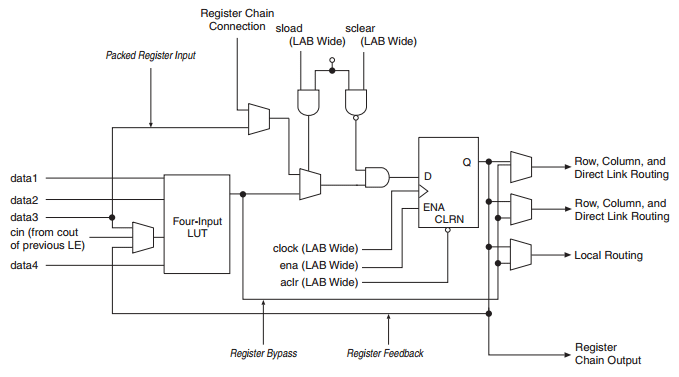
\includegraphics[width=2.5in]{LogicElement}
\caption{Cyclone III Device Family LEs in Normal Mode \cite{CycloneHandbook}}
\label{fig_LogicElement}
\end{figure}

\section{}

\section{Procedure}

\section{Results}

\section{Problems Faced \& Troubleshooting}

\section{Conclusion}


% use section* for acknowledgement
\section*{Acknowledgment}
The author would like to thank the Altera University Program for providing development boards and necessary software for work on this research.


% trigger a \newpage just before the given reference
% number - used to balance the columns on the last page
% adjust value as needed - may need to be readjusted if
% the document is modified later
%\IEEEtriggeratref{8}
% The "triggered" command can be changed if desired:
%\IEEEtriggercmd{\enlargethispage{-5in}}

% references section

\bibliographystyle{IEEEtran}
\bibliography{ieee_paper_contest}


\end{document}


